\subsection{Descripci\'on del problema}

En este ejercicio se plantea la necesidad de inspeccionar los camiones de una determinada empresa; para lo cual se puede contratar a un inspector durante un intervalo de d\'ias D. \\ 
Dados el intervalo y la cantidad de camiones c de dicha empresa, junto con la lista de d\'ias en que va a pasar cada cami\'on por el lugar donde estar\'a el inspector, la idea es elegir el d\'ia inicial de contrataci\'on tal que se maximice la cantidad de camiones inspeccionados. En caso de haber varios d\'ias iniciales que permitan controlar la misma cantidad de camiones (siempre y cuando esta cantidad sea m\'axima), cualquiera de estas opciones ser\'a correcta. \\

Por ejemplo, suponiendo que podemos contratar al inspector por 3 d\'ias consecutivos y dada una lista de d\'ias en que pasan los camiones L=[1,3,4,5,7,8,9] se puede ver en el siguiente diagrama que tanto el d\'ia 3 como el 7 son posibles respuestas.\\

\begin{figure}[h]
\begin{center}
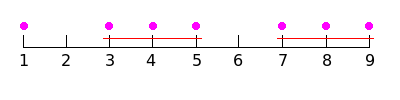
\includegraphics[scale=0.7]{./img/ej1_intervalo.png}
\caption{Ejemplo de intervalos optimos}
\end{center}
\end{figure}

\subsection{Resoluci\'on}

Para resolver el problema partimos de la idea de recorrer cada elemento de la lista de d\'ias en que pasan camiones, es decir cada posible d\'ia inicial, y a partir de ah\'i sumar uno por cada d\'ia con camiones que entrara en el rango de contrataci\'on.\\
Sin embargo, como ese algoritmo no cumple la complejidad requerida (estrictamente menor que O($n^2$)) decidimos mejorarlo reemplazando la segunda iteraci\'on sobre la lista obteniendo el \'indice del primer d\'ia con camiones fuera del rango de contrataci\'on (en $O(log(n))$) y rest\'andoselo al \'indice del primer d\'ia de contrataci\'on. De esa forma sabemos cu\'antos camiones ser\'ian inspeccionados en ese per\'iodo.\\\
As\'i, llegamos a un algoritmo que hace lo siguiente:
\begin{itemize}
\item poner m\'aximo = 0
\item poner i = 0
\item mientras i<long(listaDias)
\begin{itemize}
	\item poner ultimoDia = listaDias[i] + rangoContratacion - 1
	\item poner primeroFueraRango = indice del primer elemento mayor a ultimoDia
	\item poner inspeccionados = primeroFueraRango - i
	\item si inspeccionados > m\'aximo entonces poner m\'aximo = inspeccionados
	\item poner i = i + 1
\end{itemize}
\item devolver m\'aximo
\end{itemize}

En nuestra implementaci\'on la forma de obtener el $indice del primer elemento mayor a ultimoDia$ es utilizando el m\'etodo upperBound, que devuelve un iterador al primer elemento mayor al indicado. Con eso calculamos el \'indice de dicho iterador y lo usamos luego para restarlo con el \'indice actual y saber cu\'antos elementos hay entre ambos l\'imites.\\

Como tipo de datos elegimos:
\begin{itemize}
\item Arreglo: para la lista de d\'ias. Este tipo de datos nos permite: 
\begin{itemize}
 \item ordenar en O(n*log(n))
 \item buscar primer elemento mayor en O(log(n)+1)
 \item y nos da la ventaja extra de los \'indices, que nos permiten saber c\'uantos elementos hay dentro de un rango con una simple resta de $fin$ menos $inicio$.
\end{itemize}
\end{itemize}

\subsection{Demostraci\'on de la resoluci\'on}

Para ver que el algoritmo propuesto resuelve el problema de obtener el m\'aximo de camiones inspeccionados vamos a abstraernos del problema concreto y vamos a plantearlo de la siguiente manera: dada una lista de enteros positivos y un offset, queremos encontrar, la sublista m\'as larga de elementos tal que est\'en entre x (que puede ser cualquier entero positivo) y x + offset - 1 inclusive.\\

Llamemos n a la cantidad de elementos de la lista y o al offset.\\
Antes de empezar ordenamos la lista, ya que inicialmente podr\'ia estar desordenada; as\'i que a partir de ahora vamos a asumir que tenemos una lista ordenada de manera creciente de enteros positivos. \\ \\

Para comenzar notemos que, de todo el universo de posibles intervalos, consideraremos s\'olo los que comienzan con cada elemento de la lista; es decir que si nuestra lista es [1, 3, 5, 6] y nuestro rango es 2, s\'olo vamos a mirar los intervalos [1,2], [3,4], [5,6] y [6, 7].\\ \\

Demostremos entonces que con los intervalos que estamos considerando alcanza ya que entre ellos hay al menos uno que tiene la sublista m\'as larga.\\
Dados un offset $off$ y una lista ordenada de manera creciente $l$ y sea $S$ el subconjunto de intervalos que vamos a considerar, expresada como: \\
\begin{center}
$ S = \left\lbrace s_i = \left[ e \rightarrow l | l_i \leq e \leq l_i + off - 1 \right] \right\rbrace \forall 1 \leq i \leq long(l) $ 
\end{center}
Es decir, es un conjunto de listas tal que todos los elementos de cada lista $s_i$ pertenecen a $l$ y est\'an dentro del rango $l_i$-$l_i + off - 1$. \\
Supongamos ahora que existe una lista ordenada $s'$ que cumple con lo pedido y que es \'optima.\\
Supongamos adem\'as que esta lista \'optima no est\'a en S; es decir que no est\'a siendo considerada en nuestra resoluci\'on.\\
Sabemos que, como la lista es finita y los n\'umeros que pueden entrar en los intervalos est\'an ah\'i, entonces \\
\begin{center}
($\forall$ elem $\in$ s') elem $\in$ l, \\
\end{center}
y en particular, \\
\begin{center}
$s'_1$ $\in$ l. \\
\end{center}

Adem\'as, como la lista est\'a ordenada y cumple con la condici\'on de que todos sus elementos est\'an dentro de un rango determinado por $inicio$-$inicio + o - 1$\\
\begin{center}
($\forall$ elem $\in$ s') $s'_1 \leq$ elem $\leq inicio + off - 1$.\\
\end{center}

Notemos ahora que $inicio$ $\leq$ $s'_1$, es decir que \\ 
\begin{center}
$inicio$ $\leq$ $s'_1$ $\Leftrightarrow$ $inicio + off - 1$ $\leq$ $s'_1 + off - 1$
\end{center}
Porque, recordemos, se trata de enteros positivos, con lo cual vale la desigualdad.\\

Miremos ambos casos:
\begin{itemize}
\item inicio + off = $s'_1$ + off. En este caso pertenecer\'ia a S, ya que inicio = $s'_1$ y $s'_1$ es un elemento de l.
\item inicio + off - 1 < $s'_1$ + off - 1. En este caso el per\'iodo comienza antes que $s'_1$, pero el primer elemento de l que entra en el rango es $s'_1$, con lo cual ninguna de las listas de S se est\'a perdiendo elementos previos a $s'_1$. Por otro lado, llamemos $s_i$ a la lista de S que comienza con $s'_1$; como $inicio + off - 1$ < $s'_1$ + off - 1, podemos deducir que a $\leq$ $ s_i$. Ac\'a llegamos a una contradicci\'on: no puede haber una lista \'optima que no est\'e en S.
\end{itemize}

Una vez probado lo anterior, es trivial saber que comparando uno a uno los tama\~nos de las listas de S vamos a encontrar cu\'al es \'optima.\\

\subsection{Complejidad del algoritmo}

Analizaremos a continuaci\'on la complejidad del algoritmo propuesto utilizando un pseudoc\'odigo simplificado como gu\'ia.

\begin{itemize}
\item ordenar listaDias, $O(n*log(n))$
\item para cada d\'ia en listaDias, $O(n)$
\begin{itemize}
	\item poner ultimoDia = d\'ia + rangoContratacion - 1
	\item poner primeroFueraRango = buscar(ultimoDia, listaDias), $O(log(n))$
	\item poner inspeccionados = primeroFueraRango - i
	\item si inspeccionados es mayor que m\'aximo poner m\'aximo = inspeccionados
\end{itemize}
\end{itemize}

Decimos que ordenar la lista toma O(n*log(n)) ya que en nuestra implementaci\'on usamos std::sort.\cite{sort}\\
Lo mismo pasa cuando decimos que encontrar el primero fuera de rango toma $O(log(n))$, para lo cual usamos std::upper\_bound.\cite{upper} \\

\newpage 

\subsection{Codigo fuente}

\lstset{language=C++,
                basicstyle=\ttfamily\footnotesize,
                keywordstyle=\color{blue}\ttfamily,
                stringstyle=\color{red}\ttfamily,
                commentstyle=\color{green}\ttfamily,
                morecomment=[l][\color{magenta}]{\#},
                breaklines=true
}
\begin{lstlisting}

typedef std::vector<int> LCamiones;
typedef pair<int, int> intervalo;

intervalo resolver(LCamiones& c, int periodo){
	
	int inicio = 1;
	int maxInspec = 0;
	intervalo resultado = intervalo();
	//vector<int>::iterator itCamiones;


	// Ordeno la lista de camiones en O(n*log(n))
	// http://www.cplusplus.com/reference/list/list/sort/
	sort(c.begin(), c.end());

	vector<int>::iterator ultimoCamion;
	int inspecTemp = 0;
	int cantCamiones = int(c.size());
	int finContrato;
	int ultimoVisto = 0;
	int index;

	// Recorro los dias en que pasan camiones
	for(int i=0;i<cantCamiones;i++){
		
		// me fijo si el ultimo que verifique no es igual al actual en caso de que hayan repetidos
		if(ultimoVisto != c.at(i)){
			// Primer dia fuera del rango
			finContrato = c.at(i) + periodo - 1;
			cout << "fin contrato: " << finContrato << endl;
			
			// Obtengo el primer camion fuera del rango O(log2(N)+1) donde N es la distancia entre inicio y final
			// http://www.cplusplus.com/reference/algorithm/upper_bound/
			ultimoCamion = upper_bound(c.begin(), c.end(), finContrato);
			cout << "primero fuera de rango: " << *ultimoCamion << endl;
			
			index = ultimoCamion - c.begin();
			inspecTemp = index - i;
			cout << "camiones: " << inspecTemp << endl;

			// Si encontre un inicio mejor(o igual) reemplazo el anterior
			if(inspecTemp >= maxInspec){
				maxInspec = inspecTemp;
				inicio = i;
			}
			inspecTemp = 0;
		}
		ultimoVisto = c.at(i);

	}

	resultado.first = c.at(inicio);
	resultado.second = maxInspec;
	
	return resultado;
}

\end{lstlisting}

\subsection{Casos de prueba}

Como casos de prueba para el algoritmo elegimos inputs de los siguientes tipos:

\begin{itemize}
\item Caso en el que el per\'iodo de contrataci\'on es mayor al del rango en que pasan los camiones. El d\'ia inicial debe ser el d\'ia en que pasa el primer cami\'on y la cantidad de camiones inspeccionados es igual a la cantidad de camiones.
\item Caso en el todos los camiones pasan el mismo d\'ia. El d\'ia inicial debe ser el d\'ia en que pasan los camiones y la cantidad es igual a la cantidad de camiones.
\item Caso en el que pasa un solo cami\'on por per\'iodo posible. El d\'ia inicial debe ser el d\'ia en que pasa el \'ultimo cami\'on y ese debe ser el \'unico inspeccionado.
\item Otros casos sin ninguna particularidadd a mencionar.
\end{itemize}	

Se pueden correr los mismos casos y verificar que funcionan en el directorio /ej1 dentro del trabajo entregado, ejecutando ./ej1 < prueba.txt.

\subsection{Performance}

Para realizar el testeo de performance creamos test.cpp, el cual genera casos de test pseudo-aleatorios, determinados por una semilla, la cual se pasa como parametro al ejecutable 'test', por ejemplo: ./test 5.

Este crea 100 casos de prueba con, como dijimos, una cantidad de d\'ias en la que pasar\'a el inspector entre 1 y 100.000, un n\'umero de camiones entre 1 y 10.000.000, y el d\'ia en el que pasar\'a cada cami\'on entre 1 y 10.000.000, todos pseudo-aleatorios.

En este caso no se evalualon casos bordes porque el algoritmo tiene como complejidad del peor caso limitado por el algoritmo de ordenamiento que se utiliza sobre los d\'ias que pasan los camiones que es de O(n*log(n)) donde n es la cantidad total de camiones.
Luego se busca n veces el primer cami\'on fuera del rango de d\'ias de contrataci\'on del inspector y esto tiene una complejidad acotada por O(log(n)+1) donde n es la cantidad de d\'ias de contrataci\'on.

\begin{center}
\begin{figure}[h!]
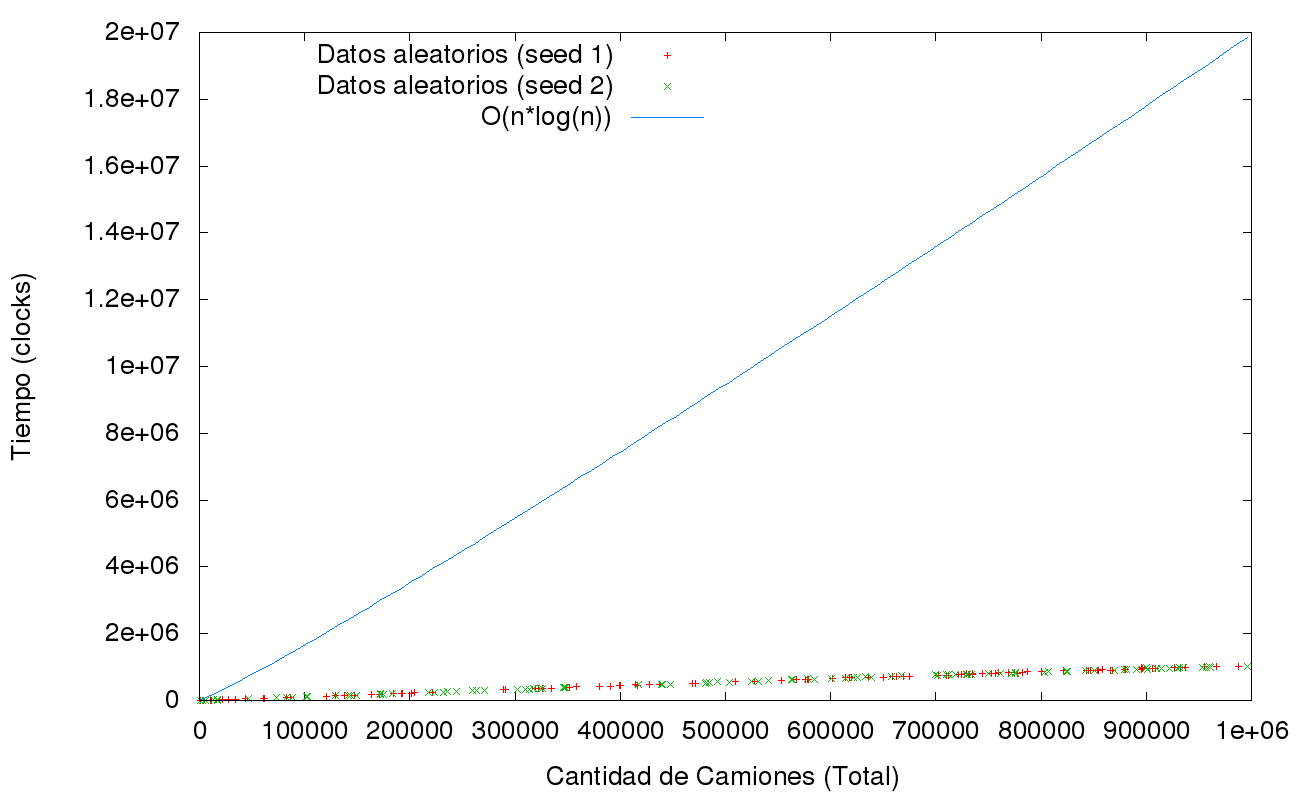
\includegraphics[scale=0.4]{./img/ej1_chart.png}
\caption{Tiempo transcurrido por eleccion de periodo de contratacion del inspector}
\end{figure}
\end{center}

Como muestra el gr\'afico, el algoritmo presenta tiempos de ejecuci\'on mucho mas \'optimos que la cota propuesta de $O(n*log(n))$.
